% !TEX root = ../../my-thesis.tex

\graphicspath{{./content/conclusion/fig/}}

\chapter{Discussion}
\label{sec:conclusion}

\cleanchapterquote{To be but one with all living things, to return, by a radiant self-forgetfulness, to the All of Nature.}{Friedrich Hölderlin (1770-1843)}{}


Understanding biological and economic systems involves the underpinning of general organizational principles at the origin of invariance (\cite{Levin2002}, \cref{fig:forward_inverse_modelling}).
% 
Aiming at advancing our understanding of eco-evolutionary dynamics in biological and economic systems, this thesis contributed to
% 
\begin{mylisti}
    \item a general understanding of the role of eco-evolutionary processes in shaping the dynamics of biological populations structured in complex landscapes (\cref{chap:diff-in-graphs}),
    \item the quantification of the effect of eco-evolutionary processes on the dynamics of economic systems at the country level (\cref{chap:econobiology}),
    \item methodological advances in the forward and inverse modelling of eco-evolutionary dynamics (\cref{chap:diff-in-graphs,chap:mini-batching,chap:nonlocalPDE}).
\end{mylisti}
% 
In the following, I discuss the chapters of my thesis collectively within the broader context of their contribution to our current understanding of the dynamics of biological and economic systems, and how they advance the current eco-evolutionary modelling paradigm. I further highlight current limitations, and propose future research directions.

\section{Contributions}

% \subsection{Advancing our fundamental understanding of eco-evolutionary processes in biological and eocnomic systems}

\subsection{Linking eco-evolutionary processes to patterns of differentiation}

Phenotypic differentiation arises from feedbacks between population dynamics, dispersal and mutations \citep{hamilton2021population}, and \cref{\chapi} determines how these feedbacks are modulated by landscape features.
% 
Mutations act upon individual organisms, and result in drift in finite size populations, causing stochastic variations in the allelic proportions and phenotypes of biological populations \citep{Slatkin1987a}.
% \cref{\chapi} contributed to advance our understanding on how eco-evolutionary processes and population structure influence population dynamics and phenotypic evolution in biological systems.
% 
% In finite size populations, mutations result in "drift" \citep{Slatkin1987a}, causing stochastic variations in the allelic proportions and phenotypes of biological populations. 
% 
In geographically structured population, drift results in patterns of neutral differentiation \citep{Slatkin1987a}, where isolated populations are characterized by differentiated allelic proportions and phenotypes. 
% 
Dispersal tends to reduce neutral differentiation \citep{Slatkin1987a}, and this effect is modulated by landscape connectivity \citep{Wright1943,McRae2006,McRae2007} through the mechanism of "isolation by limited dispersal" \citep{Orsini2013}. By increasing the dispersal ability of organisms, landscape connectivity decreases neutral differentiation \citep{Lande1991}.
% 
When landscapes present heterogeneous habitats, natural selection can supplement the effect of genetic drift and increase the sole effect of stochasticity on differentiation \citep{fisher1958genetical}. Under this scenario, local environment conditions select individuals with traits that provide them higher fitness \citep{Gaither2018}. At the population level, this results in populations adapting to their local environment, a mechanism coined "local adaptation" \citep{Kawecki2004} and resulting in patterns of "adaptive differentiation". 
% 
% This results in adaptive differentiation, and is regarded as one of the most important factors govening species richness gradients \citep{Kawecki2004}.
% 
Adaptive differentiation is hindered by dispersal, which prevents local adaptation by destabilizing the evolution of traits towards the optimal \citep{Meszena1997,Debarre2013,Mirrahimi2020}.
% 
% confounded by genetic drift, opposed by natural selection due to tempoeral envionrmental variability, and constrained by loack of genetic variation of by the genetic architecture of underlying traits \citep{Kawecki2004}. TODO: this may go in the perspective and limitations
% 
% Specifically, ref. \citep{Mirrahimi2020} presents a condition for local adaptation, where populations can locally adapt if the dispersal intensity $m$ is below a certain threshold involving the strength of natural selection $s$ and the strnegth of habitat heterogeneity $\theta$,
% \begin{equation}\label{eq:mirr_disp}
%     m < 2s\theta^2.
% \end{equation}
% 
While adaptive differentiation concerns traits under selection, it undirectly affects the differentiation of neutral traits, that are co-evolving with traits under selection through linkages \citep{Billiard2015,Lepers2021}. This results in turn to the mechanism of "isolation by adaptation", where habitat heterogeneity, rather than landscape connectivity, increases neutral differentiation \citep{nosil2008}. 
% 
Simple mechanisms resulting in neutral and adaptive differentiation are identified, but how they are modulated by eco-evolutionary feedbacks and landscape complexity is unclear. %TODO: unclear

In \cref{\chapi}, I demonstrate a novel mechanism, involving the process of intra-specific competition, that considerably affects neutral differentiation. Through the creation of unbalanced migration fluxes which increases the intensity of competition in highly connected populations, heterogeneity in connectivity reduces gene flow and reinforces neutral differentiation. %Through the accumulation of incompatibilities over time \citep{Dobhsanski}, this mechanism could lead to speciation over time, and contribute to the high diversification in mountain regions \citep{Rahbek}.
% 
I also investigate the mechanism of local adaptation in complex landscapes, where habitat connectivity is irregular. I show that the complexity of habitat spatial distribution can be reduced to a measure of habitat spatial auto-correlation, coined the "habitat assortativity". Landscapes characterised by a high habitat assortativity support populations that are systematically better adapted than in landscape with low assortativity. Specifically, I provide an analytical condition for local adaptation  (\cref{eq:xxx}), that sheds light on how it relates to dispersal intensity, selection strength, habitat heterogneity, and habitat assortativity.

Because habitat assortativity affects local adaptation, is must also affect neutral differentiation throuh the mechanism of isolation by adapation. Closing the loop, I demonstrate that habitat assortativity affects neutral differentiation through two antagonistic effects. By favoring local adaptation, it promotes isolation by adaptation, therefore increasing neutral differentiation. In parallel, it also favors gene flow within clusters of similar environmental conditions, decreasing isolation by limited dispersal. This results in habitat assortativity decreasing neutral differentiation for low dispersal intensity, and increasing neutral differentiation for high dispersal intensity.
% 
This complex feedback is essential to understand population differentiation in complex landscapes.
% 
I provide a graphical summary of the feedback mechanisms shaping neutral and adaptive differentiation identified in \cref{\chapi} in \cref{fig:summary_diff-in-graph}. Overall, \cref{\chapi} establishes a complete map of causal pathways involved in the phenotypic differentiation of populations structured in complex landscapes. % It extends on recent work including the interplay between ecological and evolutionary processes, and frequency dependence, hihglighting non-trivial emergent properties with large consequences on emergent patterns.

\begin{figure}[t]
    \centering
    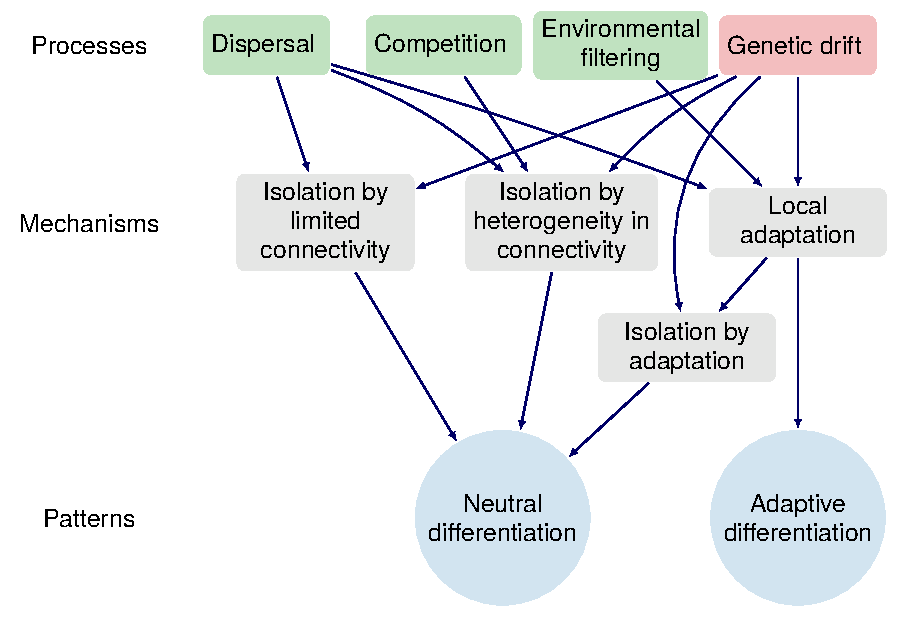
\includegraphics[width=\textwidth]{diff-in-graph.pdf}
    \caption{\textbf{Summary of the causal pathways involved in neutral and adaptive differentation, disentangled in \cref{\chapi}}. Ecological processes are displayed in green boxes, evolutionary processes are displayed in red boxes.}
    \label{fig:summary_diff-in-graph}
\end{figure}


\subsection{Linking economic patterns to eco-evolutionary processes}

% Hypotheses concerning the processes that underly economic system dynamics are numerous, and have mainly been investigated through forward modelling. Starting from empirical observations, 
% 
By confronting fine-grained empirical data and process-based models, \cref{\chapiii} bridges evolutionary economics, economic complexity and biology to better understand the endogenous drivers of economic development.
% 
%by assessing their effect on the dynamics of economic activities from data.
% 
% complements recent follows an inverse modelling approach to understand which processes are most likely shaping economic development. 
% 
Neoclassical economics and evolutionary economics seek to explain economic change with process-based models, focusing on the relationships between aggregated economic variables such as output, employment and productivity \citep{Boschma2005a}.
% 
% Neoclassical economics sugggests that exogenous drivers, such as production costs, drive the diversification of economic systems \xxx. 
% 
In particular, evolutionary economics tries to understand economic change by relating it to endogenous forces, such as interactions between firms and economic activities, and evolutionary processes acting upon them \citep{Hodgson2019,Metcalfe2006}.
% 
% Exogenous drivers, such as technological change \xxx, economic institutions \xxx, and production costs \citep{Boschma2005a} have been proposed, but 
% 
In contrast, complexity economics uses fine-grained empirical data to investigate economic change \citep{Hidalgo2021}. Instead of process-based models, dimensionality reduction techniques are used to process the data and predict variations in national income \citep{Mitchell}. 
% 
% One of the major contribution of complexity economics is to provide a metric that can predict economic development \citep{Taschella}, and the field is now concerned with understanding the factors underlying this factor.
%
While a current concern in evolutionary economics is to test the explanatory power of the proposed process-based models \cite{Hodgson2019}, complexity economics seeks to unfold the causal processes underlying the success of the dimensionality reduction technique \citep{Hidalgo2021}.

% 
% \cref{\chapiii} provides a novel understanding of the role of eco-evolutionary processes in economic systems. 
% 
\cref{\chapiii} confronts process-based models and data to underpin the processes responsible for economic change.
% 
Our approach relies on deep connections between processes acting upon economic activities and biological populations.
% 
Analogously to biological populations that are characterized by genes, economic activities are characterised by organizational routines \citep{NelsonWinter}, which experience evolutionary processes and define how they engage in ecological processes \citep{NelsonWinter}.
% 
% This connection is justified by evolutionary economics, which argues that similarly to genes, organizational routines are at the core of economic entities and experience ecological and evolutionary processes.
% 
As a result, economic activities can be considered as autonomous entities, which dynamics is determined by its characteristics and the processes acting upon them \citep{Boschma2005a}.
% 
The temporal dynamics of economic activities contain signatures, i.e. distinctive temporal variations and couplings, left by the most important processes at stage.
% 
Population dynamic models, combined with inverse modelling methods, can therefore be used to recover the role of the eco-evolutionary processes on the dynamics of economic systems, extracting this information from signatures in historical dynamics data.

%%
Specifically, \cref{\chapiii} explores the effect of processes involving positive and negative interactions between economic activities, spatial transfers, and economic activity transformations, on the dynamics of economic activities at the national scale.
% 
% \cref{\chapiii} seeks to test whether the dynamics of economic activities can be explained by different types of interdependencies, including positive \xxx and negative interactions \xxx, spatial transfers \xxx, and economic transformations \xxx.
% 
Using population dynamic models capturing the different interdependencies, \cref{\chapiii} provides empirical evidence that economic activities engage in positive interactions, and benefit from spatial transfers of knowledge and routines.
% 
Positive interactions may arise from a variety of processes proposed in the evolutionary economic literature, such as supply chains \citep{Ozman2009,Saavedra2009a} and knowledge spillovers \citep{Menon2015}. 
% 
Its support implies the dynamics of economic activities are highly inter-dependent, and suggest that diversity promotes economic development \citep{Hidalgo2018}.
% 
The support for spatial transfers implies that transfers of knowledge and organisational routines \citep{Zahra2000,Zahra2000,RogersEverettM2003DoI,Boschma2008} have a considerable effect on economic activities. Nevertheless, discrepancies in the strength-of-evidence obtained for spatial transfers across countries highlight that some countries are overall more akin to spatial transfers than others, which may be explained by differences in cognitive, organizational, social, institutional or geographic proximities across countries \citep{Boschma2005}.
% 
I provide a graphical summary of the mechanisms evidenced in economic systems in \cref{\chapiii} in \cref{fig:summary_econobio}. Overall, \cref{\chapiii} evidences that, akin to biological systems, processes of interaction and dispersal shape the dynamics of economic systems at the country scale.

\begin{figure}[t]
    \centering
    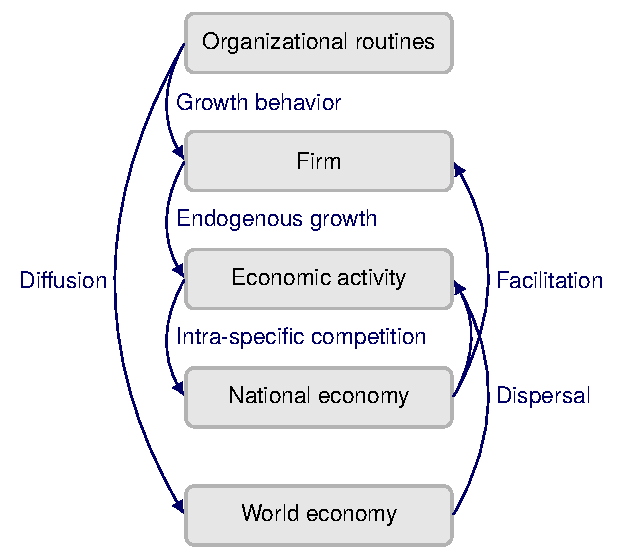
\includegraphics[]{econobio.pdf}
    \caption{\textbf{Summary of the eco-evolutionary processes evidenced in \cref{\chapiv}, and how they affect the different organizational levels in economic systems}.}
    \label{fig:summary_econobio}
\end{figure}

% 
% The dynamics of economic activities contains signals from the many complex processes that underpin them, this approach enables to extract the effect of economic processes through their 

% for the diffusion of countries through the product space, explaining technological lock out.
% 
% by using data and dimensionality reduction technique to leverage these assumptions \citep{Taschella},

\subsection{Advances in the modelling of realistic spatial and phenotypic structures}

\Cref{\chapi,\chapiv} deliver new approaches to incorporate important features of empirical systems within eco-evolutionary models.
% 
% \Cref{\chapi,\chapiv} provide new tools to better understand mechanisms resulting from ecological and evolutionary processes, and their interplay, in the context of realistic population structures and phenotypic distributions.
% 
% Population structure
Evolutionary dynamics have been traditionally studied in the context of regular population structures \citep{LiebermanHauert2005}.
% 
For instance, to investigate differentiation in biological populations, \cite{Slatkin1973,Slatkin1978,Kirkpatrick1997,Polechova2015,Polechova2018,AndradeRestrepo2019,Doebeli2003,Meszena1997,Yeaman2011,Debarre2013,Mirrahimi2020} consider regular spatial structures, missing the effect of spatial complexity on the underlying mechanisms.
% 
Biological habitats differ in their connectivity \citep{Dale2010}, and economic entities are structured through complex networks \citep{Schweitzer2009}. \cite{LiebermanHauert2005} and subsequent studies of "evolutionary dynamics on graphs" (e.g., \cite{Tkadlec2019}) show that this complexity affects the interplay between selection and drift. However, evolutionary dynamics on graphs does not consider eco-evolutionary feedbacks \citep{Govaert2019}.
% 
Thus far, models that capture eco-evolutionary feedbacks together with realistic, complex population structures were missing.

Another important feature of biological populations that may affect their dynamics is the variety of traits that characterize them \citep{Doebeli2011}. While a vast majority of the work on eco-evolutionary feedbacks has focused on the evolution of scalar phenotypes \citep{Doebeli2011}, in most organisms, many phenotypic properties combine in complicated ways to determine ecological processes \citep{Doebeli2014}.
% 
For instance, \cite{Doebeli2011} shows that the consideration of multiple traits is likely to generate more diversity than expected with one dimensional models.
% 
% \Cref{\chapi} also demonstrates that the co-evolution of traits proved to have genuine consequences on differentiation, pointing towards the inclusion of multiple traits to understand the dynamics of ecological interactions.
% 
Trade-offs in traits is also an essential feature shaping the evolutionary dynamics of biological populations, with consquences on the dynamics of e.g. cancer cell evolution \citep{Fiandaca2021} and plankton dynamics \citep{LeGland2020}.
% 
Yet the simulation of eco-evolutionary models capturing the evolution of high dimensional phenotypic distributions is tremendously difficult, since the numerical cost of traditional methods grows exponentially in the number of dimensions of the phenotypic space \citep{Bellman1957}. 
% 
% Novel numerical methods have been proposed to simulate high dimensional models, but they could not handle non-local terms, which capture non-local interactions between microscopic agents.

From first principles, \cref{\chapi} derives a stochastic individual-based model capturing eco-evolutionary feedbacks in populations structured in complex landscapes and high dimensional phenotypic space, and \cref{\chapiv} provides tools to efficiently simulate a deterministic approximation of the model in high phenotypic dimensions.
% 
% TODO: this part does not work really well
%% individual-based model
The individual-based model presented in \cref{\chapi} involves the combination of graphs and hig dimensional phenotypic spaces, together with eco-evolutionary feedbacks, to model population structures. The model can readily be generalized to include other processes (see \cref{sec:SI-comp} for an extended variant with trait-based competition), and the Julia library \textbf{Evoid.jl} \cite{Evoid.jl}, written to run the numerical experiments in \cref{\chapi}, already implements a generic version of the model. %(), 
% 
As such, the model presented in \cref{\chapi} and the Julia library \textbf{Evoid.jl} may be used to investigate other questions involving complex population structures \cite{LiebermanHauert2005} and the co-evolution of characteristics \citep{Doebeli2011}.
% 
%% PDE
Reproducing the discrete and stochastic nature of ecological and evolutionary processes \citep{Champagnat2006}, numerical simulations of individual-based model may not provide a general understanding of system investigated \citep{Lyon2016}, and cannot be scaled to simulate large systems involving millions of individuals \cite{deangelis2005individual}. Yet, the individual-based model proposed in \cref{\chapi} is mathematically tractable under simplifying assumptions, and can be efficiently simulation with a deterministic PDE approximation.
% 
Tractability allows to obtain analytical insights on how structural properties affect macroscopic population under simplifying assumptions (\cref{\chapi}).
% 
The PDE approximation, combined with the numerical methods presented in \cref{\chapiv}, further allow efficient simulations. 
% 
The numerical methods proposed in \cref{\chapiv} are now implemented in the Julia library \textbf{HighDimPDE.jl} \citep{HighDimPDE}, a registered Julia package belonging to the SciML organisation \citep{SciML}.
%% 
The user interface respects standards from the SciML organisation, meaning that Julia users can easily adopt it.
%
The package aims at hosting many more solver algorithms that break down the curse of dimensionality, and has, as of September 2022, already received contributions from 5 independent developers (see \cite{https://github.com/SciML/HighDimPDE.jl/graphs/contributors}). These contributions may greatly enhance \textbf{HighDimPDE.jl} over the years, promising efficient simulations of eco-evolutionary models.
% 
%% Conclusion
% The combination of analytical insights and numerical simulations can help to elucidate the links between microscopic processes and macroscopic properties \citep{Levin}.
% 
Together, \cref{\chapi,\chapiv} deliver novel tools to advance our understanding on the effect of the complexity of population and phenotypic structures on eco-evolutionary dynamics in complex adaptive systems.


\subsection{Advances in inverse modelling for identifying eco-evolutionary processes in empirical systems}

Our understanding and prediction of eco-evolutionary dynamics in biological and economic systems critically depends on the confrontation of process-based models with empirical data \citep{Pelletier2009,Hidalgo2021}.
% 
% \cref{\chapii,\chapiii} develop and test a novel inverse modelling method that allows to estimate parameter values and support of complex eco-evolutionary models from time-series data.
% 
The most celebrated inference methods for inverse modelling in biology are Bayesian inference methods with Markov Chain Monte Carlo \citep{Lignell2013,Higgins2010,Xu2006,Fiechter2013,Rosenbaum2019} and variational methods \citep{Schartau2017}.
% 
% Bayesian inference methods with Markov Chain Monte Carlo \xxx and variational methods \xxx have been used since the past 20 years to calibrate dynamic ecosystem models \citep{Schartau2017}.
% 
Bayesian inference methods require numerous forward model integrations \citep{Schneider2017}, and are highly affected by the number of model parameters \citep{Csillery2010}.
% 
Variational methods require the model sensitivity to its parameters \citep{Schartau2017} and are prone to converge to local minima, especially with complex models \citep{Gabor2015}.
% 
Those central issues likely explain the very limited use of inverse modelling to further our knowledge on eco-evolutionary processes in biological systems (but see \cite{Sukumaran2016,Skeels2019,Skeels2022} that use approximate Bayesian computation methods). 

%
%% Our method
\cref{\chapii} presents a novel inverse modelling framework that allows to estimate the parameter values and the support of complex eco-evolutionary models from time-series data.
% 
The framework is based on a variational method, but resolves its main shortcomings by heavily relying on automatic differentiation \citep{Rackauckas2020a}, state-of-the-art optimizers \citep{Kingma2014}, and a learning strategy based on a mini-batch method. 
% 
The use of automatic differentiation simply eliminates the effort required to obtain the model sensitivity to its parameters, and the state-of-the-art optimizers, together with the mini-batch method, ensure the efficiency and reliably of the method in handling highly nonlinear models.
% 
\cref{\chapii} takes part in an ongoing effort to blend ML and traditional models to gain scientific understanding and extrapolability \citep{Karpatne2017,Rackauckas2020a,Schneider2017,Rolnick2023,Kashinath2021,Yazdani2020,Raissi2019}. 
% 
In physical systems such as ocean and atmospheric systems, general organizational principles are known and formulated in general models. There, ML is mostly used to improve model forecast skill \citep{Schneider2017}. In contrast, general models of biological and economic systems are yet to be formulated, and methods such as the ML framework presented in \cref{\chapii} can greatly contribute to identify the general organizational principles required to reach this goal \citep{Karpatne2017}. 
% 
By contrasting competing hypotheses embedded in alternative models, \cref{\chapii,\chapiv} provide concrete examples, both with synthetic and empirical data, that the inverse modelling framework in \cref{\chapii} can successfully elucidate eco-evolutionary mechanistic pathways.
%% 
Integrating the practical constraints of current biological datasets \citep{Dornelas2018}, the inverse modelling framework may also be relevant for providing forecast ability to existing eco-evolutionary model \citep{Norberg2012}, and help to anticipate the response of ecosystems to climate change \citep{Urban2016}.
% 
Built thanks to the composability of the celebrated differential equation solver \textbf{DifferentialEquations.jl} and the deep learning library \textbf{Flux.jl}, the inverse modelling framework is implemented in the multi-purpose Julia package \textbf{MiniBatchInference.jl} \citep{MiniBatchInference}, readily available to the scientific community. %\textbf{MiniBatchInference.jl} is built around the celebrated differential equation solver \textbf{DifferentialEquations.jl} and the deep learning library \textbf{Flux.jl}. As such, the use of \textbf{MiniBatchInference.jl} requires very limited efforts to any user familiar with those libraries.
% 
Together, the inverse modelling framework proposed in \cref{\chapii} successfully blends ML methods with mechanistic ecosystem models to improve our gain scientific knowledge from observation data. Concrete case examples in \cref{\chapii, \chapiii} show that it enables the testing of eco-evolutionary theories against data, can potentially help to provide better forecasts of ecosystems states \citep{Urban2016}.

\section{Limitations}

\subsection{Forward modelling}
Alternative methods to those presented in \cref{\chapi,\chapiv} may be more appropriate for the forward modelling of eco-evolutionary dynamics.
% 
While individual-based models are interesting tools to investigate stochastic drift in finite size populations, the Gillespie algorithm \citep{Gillespie1976} used to simulate the individual-based model in \cref{\chapi} is computationally intensive, and requires to compute the fitness of all individuals at each birth or death event, which depends on the characteristics of all the other individuals. The resulting computational complexity scales poorly with the number of individuals involved, preventing its use to model large populations. 
% 
Individual-based models can be approximated by PDE models under simplifying assumptions \citep{Champagnat2006}, which are computationally more efficient in large populations for low dimensional phenotypic spaces ($\lessapprox 3$-dimensional). 
% 
% The computational complexity of standard approximation methods grows exponentially in the number of dimensions of the phenotypic space, but 
% 
The methods presented in \cref{\chapiv} can efficiently simulate PDE models in higher dimensions (demonstrated up to 10 traits), but still suffer from a number of issues that may prevent their practical use.
% 
First, the MLP method can only provide the population number for one single trait value in one run. Consequently, the MLP method cannot characterize the total population density with a reasonable computational complexity. 
% 
In contrast, the ML-based approximation method can provide the full population density, but involves the training of many neural networks (one at each time step). This is worrying, since the training of a neural network is numerically costly, and that long simulation times may be required by practitioners. Another problem with the numerical methods proposed in \cref{\chapiv} is that they involve the tuning of meta parameters, including the choice of a measure for the integration of the non-local term ($\nu_x$ in \cref{frameworkMLP, frameworkDS}). This measure is critical for the success of the numerical simulations, but how to determine it is unclear.
% 
Together, the methods proposed in \cref{\chapiv} may require further development to be used in practice by practictioners. 

Because PDE models track the evolution of the full phenotypic density of populations, PDE models inevitably require a considerable computational effort - irrespective of the numerical method used. 
% 
Nevertheless, only the first three moments of the population density are usually of interest, namely population size, trait mean and trait variance \citep{Nordbotten2020}. 
% 
Instead of seeking to numerically approximate the full phenotypic density, moment closure approximation methods \citep{Wickman2021,Lion2022,Nordbotten2020} may be considered. Those approaches consist in approximating the population density with a Gaussian distribution. This, in turn, allows to transform the PDE problem into a system of coupled differential equations involving the time evolution of the population size (1 variable for a single species population), the mean trait values ($d$ scalar variables), and the variance-covariance matrix of the multidimensional trait density ($d^2$ variables). As such, the computational cost of this method only scales polynomially with the number of dimension ($\mathcal{O}(d^2)$), while providing the sufficient information required to investigate eco-evolutionary dynamics in high dimensional phenotypic spaces. 
% 
It is worth noting that instead of using neural networks, Gaussian functions could also be used within the ML-based method for simulating eco-evolutionary models. Equivalent to the simplifying assumption taken with moment closure methods, we expect this approach to greatly improve the computational efficiency of the ML-based method, while solving the problem of the choice of a kernel for the integration of the nonlocal term. Using Gaussian functions may considerably lower the number of iterations required in the training process, while reducing the computational cost, as they involve fewer free parameters ($d(d+1) + 1$) than neural networks ($xx$ in \cref{examplesxxx}).

Together, the proposed methods in \cref{\chapi,\chapiv} suffer from considerable computational cost, because they seek to simulate PDE models which track the evolution of the full phenotypic distribution of populations. Because only the population number, the mean and the variance-covariance matrix of the phenotypic distributions are of interest, closure approximation methods could be considered. Those methods are compatible with the ML-based method proposed in \cref{\chapiv}.


\subsection{Inverse modelling}
The inverse modelling framework proposed in \cref{\chapii} and used in \cref{\chapiii} also present pitfalls, which may favor the use of other methods to infer eco-evolutionary processes from empirical data.
%
First, the mini-batching learning strategy requires the choice of a minibatch size to ensure the convergence to the maximum likelihood estimate. This choice should be motivated by the roughness of the model likelihood landscape (see \cref{sec:XXX}), but may affect the model selection process:
a small batch size implies that the model goodness-of-fit is evaluated on the fast dynamics of the data, but the resulting support could differ, were the model fitted with a higher minibatch size. Theoretical developments are required to provide statistically justified guidance for the choice of this meta parameter. 
% 
Second, the maximum likelihood estimate of models with complex likelihood landscape may be underestimated, because not correctly identified. As a result, the model selection process may be biased towards models with easier to navigate likelihood landscapes. 
% 
Third, the information criterion-based model selection procedure used in \cref{\chapii,\chapiii} is uniquely based on a trade-off between the goodness-of-fit and the number of parameters of the model, which may not be satisfactory to characterize process-based model \citep{Clermont2015}. 
% 
% For instance, \cite{XXX} shows that the logistic map, which consists of only two parameters, can be fitted to any pattern. 
Other criterion, involving the complexity of the dynamical behavior of the model (such as, e.g., its Lyapunov exponent), could be developed.
% 
Fourth, the inverse modelling framework developed in \cref{\chapii} requires a differentiable model, a strong prerequisite that may not be met by stochastic models. 
% 
Fifth, the inverse modelling framework only provides the maximum of the posterior distribution, while the posterior distribution may be multimodal. The alternative modes may carry valuable information to consider in the model selection process \citep{Daniels2015}.%, and in this case, the consideration of the full posterior distribution, obtained with fully Bayesian methods, may be more appropriate for model selection.

% 
Alternatively, \cite{Sukumaran2016,Skeels2019,Skeels2022} employ variants of approximate Bayesian computation methods for eco-evolutionary model selection \citep{Csillery2010}. The approach consists in aggregating model simulation outputs into summary statistics, used to train classifier algorithms (e.g., random forests or neural networks) in recognizing the signatures of the competing models. Once trained, the classifier algorithms are used on summary statistics obtained from the empirical data, discriminating between the alternative hypotheses. 
% 
This approach does not require model differentiability, and is consequently more flexible than the method proposed in \cref{\chapii}. Also, the use of summary statistics can elucidate which particular feature of the empirical data is better explained by a given model. 
% 
Nevertheless, this strength is a pitfall: summary statistics necessarily reduce the information contained in empirical data, which can prevent to correctly discriminate between models \citep{Csillery2010}.
% 
Together, the minibatch inverse modelling framework in \cref{\chapii} is sensitive to the minibatch size, requires models to be differentiable, and does not provide uncertainty estimation. While approximate Bayesian computation may be a valuable alternative, it also presents restrictive shortcomings. Still, the minibatch learning strategy extends beyond the framework proposed, and could be used in combination with novel approaches in Bayesian computation to combine the best of both worlds.

\section{Perspectives}

\subsection{Development opportunities in inverse modelling}

The mini-batch method presented in \cref{\chapii} and the ML-based approximation method developed in \cref{\chapiv} offer unique development opportunities to leverage inverse modelling.
%%
The mini-batch method is relevant beyond the ML framework presented in \cref{\chapii}, and could be used within a fully Bayesian framework, where the full posterior distribution of the model is estimated. Compared to a plain vanilla Bayesian inference, using the loglikelihood formulation proposed in \cref{eq:xxx} would result in a simpler posterior distribution, potentially reducing the number of forward model integration.
% 
While this number could still be prohibitively expensive for Bayesian inference with MCMC chains (see \cref{sec:xxx}), automatic differentiation variational inference (ADVI, \cite{Morningstar2020,Gosh2021}) offers an appealing alternative. In ADVI, the posterior distribution is approximated by a Gaussian distribution \citep{Morningstar2020}, significantly reducing the number of model integration \citep{Morningstar2020}. Improving the ML framework presented in \cref{\chapii}, ADVI could capture multimodality in the model posterior distribution (by approximating the multimodal distribution with a gaussian distribution with large variance). This, in turn, could improve the robustness of model selection (\cref{sec:limitations}), and provide uncertainties estimations on the parameters.
% 
Providing uncertainty estimates while ensuring computational efficiency, Bayesian Learning via Stochastic Gradient Langevin Dynamics \citep{Welling2011BayesianLV} could also be used instead of the optimization algorithms employed in \cref{\chapiii,\chapiv}. This algorithm builds upon recent advances in Bayesian Deep Learning \citep{Wilson2020}, and interprets the iterative gradient-based optimization procedure as a Markov chain with an equilibrium distribution over the posterior distribution of the model parameters. It therefore comes with the scalability of variational methods and the interpretability of Bayesian methods, and can provide good estimates of uncertainty errors for complex models.

%%
The ML-based approximation method for high dimensional PDEs, presented in \cref{\chapiv}, could be used for inverse modelling.
% 
In \cref{sec:frameworkML}, the parameters of the PDE model are assumed fixed, but could be set as free parameters, analogously to the parameters of the neural networks used for approximating the solution. The loss function in \cref{eq:xxx} would then take the PDE model parameters as additional arguments, and include an additional term, involving the distance between the PDE model solution and the data. This term, analogous to \cref{eq:xxx} in \cref{sec:xxx}, would constrain the PDE parameters, similarly to the training of physics informed neural networks \citep{Raissi2019,Yazdani2020}.
% 
In contrast to \cite{Raissi2019,Yazdani2020}, a major advantage of this approach it to efficiently perform inverse modelling with high-dimensional dynamical models. Because Julia is a programming language with pervasive AD, this development would require little effort with the Julia library \textbf{HighDimPDE.jl}.
% 
Together, the ML methods developed in \cref{\chapii,\chapiv} offer unique opportunities to bring more robustness and efficiency to inverse modelling methods, providing uncertainty estimation and the possibility to handle high dimensional models.

% Allows to estimate the uncertainty in estimation, and localize different equally likely region in the parameter space that are likely.


% The piecewise loglikelihood function presented in \cref{\chapii} (\cref{eq:minibatch}) 


\subsection{Confronting eco-evolutionary model on spatial graphs and empirical data}

The confrontation of the predictions from \cref{\chapi} with empirical data, and the use of inference methods with the proposed eco-evolutionary model on spatial graphs, could advance our understanding of eco-evolutionary dynamics in empirical systems.
% 
\cref{\chapi} proposed topology metrics that should correlate with standard population differentiation metrics ($Q_{ST}$ metrics). Because real landscapes can be projected on spatial graphs (\xxx and \cref{fig:diff-in-graphs}), the topology metrics, together with empirical data on population differentiation (e.g., \cite{Fluerin}), could be used to verify our predictions. Discrepancies may indicate that other important processes may be involved in empirical patterns. On the other hand, a validation of our predictions could help to predict population differentiation at a global scale. These predictions could, in turn, be linked to patterns of species richness, in order to underpin how population genetics may lead to speciation over time \xxx.
% 
In the same direction, the use of the eco-evolutionary model on spatial graphs, together with paleo-climatic data \citep{HagenXXX} and inference methods, could help addressing fundamental questions on the processes involved in current biodiversity patterns. \Cref{\chapi} succinctly tests whether our predictions hold for a more general setting involving trait-based competition. Trait-based competition may be ubiquitous in biological systems \xxx, and similarly to the process of environmental filtering \xxx, can lead to diversification. An important question on the research agenda is to underpin how competition may mediate environmental filtering and promote and hamper diversification over time. This fundamental question could be adressed by embedding the competing hypotheses in alternative models, which support could be tested against data.
% 
Along shorter time scales, the eco-evolutionary model on spatial graph could be calibrated on empirical data of species distribution \xxx with the inference method proposed in \cref{\chapi}, and combined with climate scenarios \xxx to better predict how biological populations will adapt to climate change \citep{Norberg2012,Urban2016}.
% 
Together, the model developed in \cref{\chapi} and the resulting predictions, together with the ML framework presented in \cref{\chapii}, could bring insights on the actual mechanisms involved in empirical systems, and help to predict their responses to climate change. 
% may be used to characterize real landscape properties


% eco-evolutionary model on spatial graphs presented in \chapi, together with its predictions, and inverse modelling methods, could be used to advance our understanding of the processes shaping the distribution of life on Earth, and contribute to a formalization of the theory, to provide forecasts


\subsection{Econobiology, a new venue to understand economic systems, and design more appropriate governance}

The current understanding of key processes and patterns in biological systems may provide insights into general organizational principles in economic systems, and provide guidance for economic policies.
% 
The biologically inspired eco-evolutionary model presented in \cref{\chapiii} was succesful in characterizing the dynamics of economic activities. \Cref{\chapiii} therefore evidences deep connections between processes acting upon economic and biological systems. 
% 
On top of encouraging the characterization of these processes at a finer level, this calls for investigating parallels in the dynamics and organizational principles between biological and economic systems.
% 
% Results from \cref{\chapiii} 
% 
There may be connections between nutrient cycles in ecosystems \citep{Veldhuis2018} and capital cycles in economic systems \citep{King1993}, where ecological compartments and financial intermediaries develop to improve the efficiency of nutrient flows and capital allocations \citep{Odum1969}.
% 
\cite{Veldhuis2018,King1993} show that this efficiency sustains productivity and growth, but the developmental process may fail, where ecosystems stay in a state of lower maturity \citep{Margalef1963} or technological lock-in \citep{Hidalgo2009}. 
% 
What are the links between the evolution of nutrient and capital cycles, and the fundamental processes acting upon lower organization levels?
% 
% Linking structural patterns and underlying processes, \cite{Saavedra2009a} shows that the processes of specialization and interactions yield similar organizational properties in plant pollinator systems and in firms engaged in joint production.
% 
Future directions should seek to understand at a finer level the processes evidenced in \cref{\chapiii}, and understand how they may result in organizational principles at the economy level.
% 
\cite{Veldhuis2018} provides a synthesis of our understanding of how ecosystem organization emerges through self-reinforcing mechanisms, promoted by ecological and evolutionary processes acting upon producers, consumers, and decomposers. This synthesis provides an interesting roadmap, and analogous self-reinforcing mechanisms could play important roles in determining fluxes of capital in economic systems. 
% 
The quest for finding common organizational principles may help us to distinguish important differences between economic systems. Since biological systems have undergone evolution for a much longer time than economic systems, they may be more effective and resilient than economic systems. These difference may inspire economic policies.
% 
% We know that herbivores, regulating plant dynamics, play a central role in ecosystems \citep{RitchieTilman}. 
% 
% By consuming nitrogen-fixing and woody plants, they control nitrogen cycling and light, which are essential plant resources \citep{RitchieTilman}. 
% 
% For instance, they promote plant diversity, feeding on the more abundant plants and reallocating the resources through their feces \cite{Schmitz}. Diversity, in turn, leads to ecosystem productivity.
% 
% Governments may play analogous roles to herbivores, reallocating taxes through investments in research and education, or subsidizing firms \xxx.
% 
Altogether, biology may eventually help us understanding organizational principles in economic systems, and provide guidance for improving economic regulations.

%   

% \cite{Odum1969} suggested 50 years ago that ecosystem and human societies tend to follow the similar development trajectories.
% 
% Common organizational structures have also been documented at different organizational level \cite{XXX}.
% 
% Evidences of similar ecological and evolutionary processes, and organizational structures, encourage seeking for common organizing principles \citep{Olff2008}.
% 
% \cite{Veldhuis2018} provides a synthesis of our understanding of how ecosystem organization emerges through self-reinforcing processes. Such processes could play important roles in determining fluxes of capital in economic systems.
% 
% \cite{Veldhuis2018} highlights that in order to understand ecosystem organization, the link between producers, consumers, and decomposers is essential.
% 
% Similarly, I believe that to underpin the dynamics of economic systems, we need to account for more than the dynamics of economic activities, and include financial intermediaries, which, by better allocating capital, promote economic efficiency and growth \cite{King1993}. 

% These common organizational structures may be explained by common organizing principles, which are essentially ruled by ecological and evolutionary processes \citep{Veldhuis2018}.
% 
% For instance, \cite{Saavedra2009a} shows that the processes of specialization and interactions yield similar organizational properties in plant pollinator systems and in firms engaged in joint production.
% 
% Also 

% 
% More generally, are there common organizational principles that can explain dynamics and structures in biological and economic systems? \cite{Veldhuis2018} provides a synthesis of our understanding of how ecosystem organization emerges through self-reinforcing processes. Such processes could play important roles in determining fluxes of capital in economic systems.
% 
% In biological systems, we know that more species diversity is associated to more productivity \citep{Duffy2017a}. Does the diversification of an economy leads to more economic development?


% In particular, whether the processes we found are conserved at different organizational levels
% 



\section{Concluding remarks}

It is, more than ever before, urgent to better understand and forecast the dynamics of life on Earth.
% 
While we know that the global temperature on Earth will rise by 2 to 4 degrees in 2100, predictions on ecosystem states are much more uncertain. Yet obtaining more realistic ecosystem forecasts is critical to help designing adequate management of ecosystem services.
% 
Blending scientific knowledge, formalised in mathematical model, with machine learning, provides unique opportunities to quickly improve our understanding of ecosystem dynamics and provide forecasts. % Tools developed within this thesis can help doing so.
% 
Machine learning is part of the astonishing technological progress experienced by humankind in the last centuries. This progress has led us to think that we are rational beings, that have crafted singular socio-economic to create wealth. Yet it may well be that socio-economic systems are analogous to, but less efficient and resilient than, biological systems. 
% 
Realising overlaps and differences in processes shaping economic and biological systems may be extremely beneficial: we could surely take inspiration from organizational principles in biological systems, that have survived major environmental crisis for more than 3.5 billion years.
% 
To conclude, let us cite Hölderlin: "\textit{To be but one with all living things, to return, by a radiant self-forgetfulness, to the All of Nature}". 





% Understanding eco-evolutionary dynamics




% We are far from an understanding biodiversity at a planetary scale comparable to how we understand Earth’s climate. Yet, what is at stake for human societies around the world, is at a minimum comparable to those derived from climate change.


% In contrast to the Navier Stokes equations, w

% Connecting biology, economics, mathematical models and machine learning, this thesis contributed to a better understanding of eco-evolutionary dynamics in biological and economic systems.
% % 
% Mathematical models formalize our prior knowledge on , and 
% % 
% We are now better equipped for a quantitative understanding of eco-evolutionary dynamics in realistic biological systems. In particular
% % 
% In light of the results from \cref{chapi,chapiii}, I believe that the paradigm of eco-evolutionary dynamics, in combination with network to capture realistic structures 

% Approximation Bayesian Computation is a more flexible approach for inverse modelling, that bypasses exact likelihood calculations by using summary statistics \cite{Csillery2010}. Summary statistics aggregate the empirical data into informative metrics, which can the be
% contain information about the data in aggregated forms

% 
% 
% 
% \printbibliography[heading=subbibliography]
% \subsection{Blending ML and mechanistic models to learn from data}

% \subsection{Quantitative support for eco-evolutionary processes in economic systems}

% \subsection{Novel methods for the modelling of complex adaptive systems}


% \section{Limitations}

% \subsection{Limitation of PDE methods}
% \citep{Akesson2021} : PDE methods are probably not as adapted as trait based ODEs. Those simpler models can already address important questions regarding climate change.
% \citep{Tacchella2018}: In many cases, not only in economics, theoretical modelling and forecasting are not tightly related5
% . Most of the modelling efforts are
% in the direction of oversimplified representations that aim only at understanding the potential effects of a single variable, or of a lim- ited set of them, in a controlled setting

% \section{Conclusion}
% In light of the results, XXX.
% % 
% We expect XXX.

% %%
% Consequently, this thesis contributed to a better understanding of XXX.
% % 
% While recent studies have underlined the need to account for XXX, we XX.

% \section{Perspectives}

% \subsection{Toward a continuum between ML and mechanistic models}

% \subsection{Evolutionary biology to undertsand the economic patterns}


% \subsubsection*{An urgent need for better understanding and model eco-evolutionary dynamics}
% The effect of direct anthropogenic pressure, together with climate change, is rapidly affecting ecosystems \citep{Ellis2011,Midgley2019}. Ecosystems are approaching state shifts \citep{Barnosky2011,Barnosky2012,Midgley2019}, which in turn will greatly affect human societies \citep{Mooney2009}.
% %
% %% Constatation of system state shift
% % Current extinction rates are higher than would be expected from the fossil record \citep{Barnosky2011}. %Based on habitat models, \citep{Midgley2019} predicts, on the basis of mid-range climate-warming scenarios for 2050, that 15\% to 37\% of species would be committed to extinction. 
% % 
% %%
% While there is a general agreement that anthropogenic pressure and climate change will have a negative effect on the biosphere \citep{fischlin2007ecosystems}, their precise effect on ecosytem dynamics is unclear \citep{Norberg2012}. In particular, the answer to how species will adapt to increasing temperatures is uncertain due to our lack of understanding of eco-evolutionary feedbacks \citep{Norberg2012}. 
% % 
% %For instance, with global warming, species are likey to shift towards higher elevations and higher latitudes \citep{Chen2011}. Because the speed of range shifts differ between different ecological groups, climate change is expected to modify the current organization of trophic interactions \citep{Descombes2020}, affecting ecosystem functioning.
% %
% %% 
% Current projections of ecosystem states, such as \citep{Midgley2019},
% are based on habitat models, where species habitats are deducted from species occurence data, and are reprojected it given environmental predictors.
% % 
% Such approaches miss the processes of ecological interactions, evolutionary change and species dispersal \citep{Pearson2003}, that are expected to play a critical role in the evolution of the biosphere in the coming decades \citep{Norberg2012}.
% % 
% In order to mitigate the consequences of human development, it is of utmost urgency to better understand eco-evolutionary feedbacks \citep{Norberg2012}, and develop mechanistic models embedding this knowledge \citep{Urban2016}. This will in turn provide more reliable forecasts of ecosystem states \citep{Clark2001}, to help designing adequate management of ecosystem services \citep{Urban2016}.

% % \subsubsection*{Endogenous forces in economic systems}
% % Traditional approaches to economics assume the rationality of economic agents \xxx. Economic dynamics
% % % 
% % In contrast, evolutionary economics 